\documentclass[german, pt]{MTSreport}

\usepackage{comment}
% \usepackage{draftwatermark}
% \SetWatermarkText{DRAFT}
% \SetWatermarkScale{0.5}
\bibliography{listings/bibliography}


% Custom methods
\makeatletter
\newcommand{\setword}[2]{%
  \phantomsection
  #1\def\@currentlabel{\unexpanded{#1}}\label{#2}%
}
\makeatother
% End 

\title{Ermöglichung des Hardware- und Software-in-the-Loop durch die Einbindung von BaSyx und MATLAB/Simulink}
% \subtitle{Untertitel wenn nötig} % Just delete it if you don't have a subtitle
\author{Mateus Molina}
\tuklid{420495}
\semester{3}
\email{molina@rhrk.uni-kl.de}
\supervision{Dipl.-Ing. Paaranan Sivasothy\\ Prof. Dr.-Ing. Jörg Seewig}
\date{Juni 2022}
\keywords{Simulink, BaSyx, Digitaler Zwilling}

\begin{abstract}
Fill this area with your abstract
\end{abstract}

% \begin{preface}
% optional
% \end{preface}

%optional acknowledgment
%\begin{acknowledgment}
%optional
%\end{acknowledgment}


\begin{document}

\chapter{Einleitung}

\section{Motivation}
% Details über Anwendung von Simulink im Markt
Simulink wird häufig in verschiedenen Industrie-Branchen von Ingenieuren großer und kleinerer Firmen eingesetzt, um Modelle mit wiederverwendbaren Komponenten und Bibliotheken zu simulieren. \cite{enlyftSimulinkMarketShare} \cite{themathworksinc.SimulinkGettingStarted}

% Verbidung mit model basierte Entwicklung
% Verbidung mit Industrie 4.0

% Details über Anwendung von BaSys im Markt
BaSys 4.0 ist ein vom BMBF gefördertes Forschungsprojekt, das von Fraunhofer IESE gemeinsam mit 14 weiteren Partnern aus dem Bereich der Produktionstechnik entwickelt wird, um digitale Zwillinge als digitale Repräsentanzen für die Produktion zu realisieren.  \cite{fraunhofer-institutfurexperimentellessoftwareengineeringieseBaSysFlyer}

Eine Open-Source Implementierung der von BaSys festgelegten Konzepten, ist Eclipse BaSyx, ein von BaSys finanziertes Middleware, das wiederverwendbaren Industrie 4.0 Komponenten und SDK in verschiedenen Programmiersprachen bereitstellt, wobei die schnelle Entwicklung neuer Software-Komponenten ermöglicht wird. \cite{eclipsefoundationinc.BaSyxEclipsepedia}

% TODO Was für Firmen nutzen BaSyx?

% Was für Vorteilen würden sich ergeben, durch die Verbindung beider Plattformen?
% TODO #7 Hardware-In-The-Loop vs Model-In-The-Loop vs Model-Based Systems Engineering (MBSE)
Simulink zusammen mit BaSyx könnten eingesetzt werden, um Hardware-In-The-Loop leichter einzusetzen, wobei BaSyx um die Struktur der digitalen Zwillinge kümmern würde, während Simulink für das Simulieren einzelner Bauteile oder Regelung gesamter Komponenten angewandt würde.  

% Noch ein Use-Case hinzufügen

% Keine einfache Methode beider Tools zu verbinden
Nach Prüfung von verschiedenen Alternativen, Simulink und BaSyx zusammen einzusetzen, hat sich herausgestellt, dass eine Kommunikationsschnittstele zusätzliche Kenntnisse im C, REST und die innere Funktionsweise vom BaSyx voraussetzt, was ein limitierender Faktor für eine breitere Verwendung in der Industrie darstellen könnte. Eine detaillierte Rechtfertigung für das Projekt lässt sich im Kapitel \ref{verbindung_basyxsimulink} finden.


\section{Zielstellung}
Im Rahmen dieser Arbeit soll eine Simulink-Bibliothek entwickelt werden, die die Kommunikation zwischen BaSyx-Servers und Simulink ermöglicht. 

% Zusammengefasster Umfang
1. Bibliothek für Simulink
2. Demonstrator für die entwickelte Bibliothek 


% für milestone @mai
% Anforderungstabelle
\begin{table}[h]
    \centering
    \begin{tabular}{|c | c|} 
        \hline
        id & Anforderung \\ 
        \hline
        \setword{A10}{req:A10} & Soll mit einem BaSyx-Server verbinden können \\
        \hline
    \end{tabular}
    \caption{Anforderungstabelle}
    \label{table:Anforderungstabelle}
    \end{table}
% - Herleitung der Tabelle
% - Ausgabe der Marktforshcung??

Laut der Anforderung \ref{req:A10}


\section{Gliederung der Arbeit}
Im Kapitel \ref{grundlagen} wird was diskutiert.

Im Kapitel \ref{plannung_durchfuhrung} wird was diskutiert.

Im Kapitel \ref{validierung} wird was diskutiert.

Im Kapitel \ref{zusammenfassung} wird was diskutiert.
\chapter{Theoretische Grundlagen} \label{grundlagen}

\section{Simulink}
\section{Digitaler Zwilling}
\section{BaSyS und BaSyX}
\subsection{BaSys}
\subsection{BaSyx}
BaSyx benefits and use-cases

BaSys 4.0 enables the digitisation of manufacturing processes and the implementation of Industry 4.0. Eclipse BaSyx is an Open-Source reference implementation of BaSys 4.0 concepts that include common Industry 4.0 components and a Software Development Kit (SDK) that supports the development of new components. Eclipse BaSyx did originate from the BaSys 4.0 project, which is funded by the german ministry of Research and Education. The following examples highlight common Industry 4.0 use-cases that can be realized with the BaSyx middleware: 

\section{Hardware-in-the-Loop}
\section{Model-Based Systems Engineering (MBSE)}


% Soll ich diesen Abschnitt hinzufügen? 
\section{Stand der Technik}
\subsection{MatLab Production Server}

\section{Möglichkeiten Simulink und BaSyx zu verbinden} \label{verbindung_basyxsimulink}
% für milestone @mai 
% Wer würde sich dafür interessieren?
% Das wäre ein interessanter Sprechpunkt fürs Meeting
% - Wie macht man eine Marktforschung passend für diese Art von Projekten?
% - Methodologien??
% - UX??
% - Umfrage?? 

\section{REST Schnittstellen}
\section{Entwicklung von Simulink-Bibliotheken} 
\subsection{S-Functions}


\chapter{Plannung und Dürchführung} \label{plannung_durchfuhrung}
% [X] Chapter Einführung
Dieser Kapitel ist in zwei Unterkapiteln aufgeteilt, der Entwicklungsprozess und der Entwurf. Im ersteren wird darauf eingegangen, wie die Entwicklung des Projektes abgelaufen ist, mit Emphase auf Anforderungen, Betriebsmodi, funktionelle Architektur und die Softwarestruktur. Im zweiteren werden Designaspekten jeder Anforderung beleuchtet, wobei diese technisch beschrieben und mit Auszügen des Quellcodes kontextualisiert werden.  

\section{Entwicklungsprozess} \label{Entwicklungsprozess}

\subsection{Anforderungsdefinition}
\begin{figure}[H]\centering
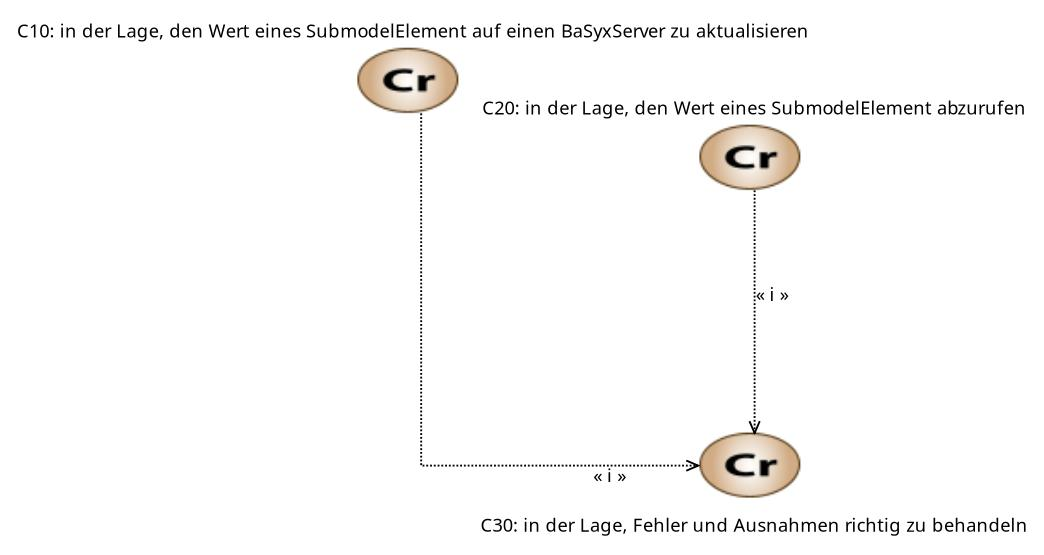
\includegraphics[width=10cm,height=10cm,keepaspectratio]{media/diagrams/CRB.jpg}
\caption{Capabilities Diagram)}
\label{fig:CRB}
\end{figure}

\subsection{Funktionale Spezifikation}

\section{Entwurf} \label{Entwurf}

% Beschreibung jedes Capabilities des Projektes
% - Problemstellung und Motivation
% - Methodologie
% - Endarchitektur
\subsection{Wrappen des BaSyx als S-Function}


\chapter{Validierung} \label{validierung}
% [X] Vorstellung des Kapitels

Im folgenden Kapitel wird der beispielhafte Anwendungsfall vorgestellt, der die Umsetzung der Anforderungen veranschaulichen soll. Im ersten Teilkapitel wird dessen Aufbau besprochen, während im zweiten und letzten ein Überblick bezüglich der Erwartungen und der im Beispiel erzielten Ergebnisse gewonnen wird. 

\section{Beispielszenario}

Für das Testen des Systems wurde ein Beispielszenario entwickelt, welches die Funktionalität der in der Arbeit entwickelten Bibliothek aufzeigt. Dafür wurde ein vereinfachtes Beispiel des \textit{Condition-Monitoring} realisiert, bei dem die Funktionsweise eines Temperatursensors und des Hauptantriebssystems einer Pressmaschine in Simulink nachgebildet und deren digitale Zwillinge in einem \textit{BaSyx}-Server gespeichert werden. Die Temperaturdaten werden letztendlich in einem in Simulink realisierten Dashboard dargestellt.

% [X] @tagline use-case besser beschreiben
Dies bezieht sich auf einen häufigen Anwendungsfall in der Industrie, in dem der Zustand einer Maschine überwacht werden soll, um möglich Ausfälle und Fehler frühzeitig zu erkennen. Im ausgewählten Szenario wirken die Daten aus dem Temperatursensor als Metrik für die Entscheidungsfindung, ob sich die Stanze im normalen Betriebzustand befindet, wobei eine Überschreitung eines voreingestellten Schwellenwerts im einfachsten Fall zu einer Warnung auf dem Dashboard führt. 


\subsection{Setup der \textit{BaSyx}-Infrastruktur mit \textit{Docker}}

% [X] Docker-Compose Auszug aufbau  usw
Beide für das Beispiel verwendeten Registry- und AAS-Server nehmen die verfügbaren \textit{docker containers} von \textit{BaSyx} im Anspruch. Bei Nutzung von \textit{docker-compose} wird eine schnelle Bereitstellung der beiden notwendigen \textit{containers} möglich. In Codeauszug \ref{code:docker-compose} ist der Aufbau der im Beispiel eingesetzten Konfigurationsdatei für \textit{docker-compose} abgebildet. Bei Nutzung von \textit{Docker-Containers} wird vermieden, dass erst eine komplexere Anwendung in Form einer \textit{Java}-, bzw. \textit{C}-App erstellt werden muss. 

% [X] @tagline instead of running a complex java app the user can essentially start the basyx cont in order to have basyx running as a service in the machine

% [X] Change listing package to minted to support YAML
\begin{codeblock}{YAML}{docker-compose}{Auszug aus der Datei docker/docker-compose.yml}
    # docker/docker-compose.yml
    version: '2.1'
    services:
    registry:
        image: eclipsebasyx/aas-registry:1.1.0
        container_name: registry
        volumes:
            - ./conf/reg-config:/usr/share/config:z
        ports:
            - 8082:4000

    aas:
        image: eclipsebasyx/aas-server:1.1.0
        container_name: aas
        volumes:
            - ./conf/aas-config:/usr/share/config:z
        ports:
            - 4001:4001
\end{codeblock}

Zu Beginn lädt der AAS-\textit{container} die in Abb. \ref{fig:aasxexplorer} dargestellte AAS. Diese enthält zwei \textit{Submodels} für die vereinfachte Abbildung von Hauptantrieb und Temperatursensor. Diese weisen wiederum je ein \textit{SubmodelElement} auf, die entsprechend zur Darstellung der aktuellen Last am Antriebe und des aktuellen erfassten Temperaturwertes dienen.  

\img{10cm}{media/presse/aasxexplorer.png}{aasxexplorer}{Bildschirmaufnahme der Verwaltungsschalle auf AASX Package Explorer}



\subsection{Aufbau}

Das Simulink-Modell (Abb. \ref{fig:simupresse}) besteht aus 4 Teilsystemen:
\begin{enumerate}
    \item Last: aktualisiert den Wert vom \textit{Hauptantrieb/last SubmodelElement} mit dem Wert einer Schiebekomponente.
    \item Hauptantrieb: bildet die Funktionsweise des Hauptantriebes nach und gibt den aktuellen Wert der Temperatur am Kontakt zwischen Antrieb und Sensor an.
    \item Temperatursensor: bildet die Funktionsweise des Temperatursensors und schickt den abgetasteten Wert an  \textit{TempSensor/temperatur SubmodelElement}.
    \item Dashboard: erhält und verarbeitet die Daten aus dem  \textit{TempSensor/temperatur SubmodelElement} und ermöglicht \textit{Monitoring} über einen Graph
\end{enumerate}  

Beim Einstellen des Schiebers im Last-Teilsystem ändert sich die Temperatur des Hauptantriebs. Dieser Effekt wirkt sich auf das Temperatursensor-Teilsystem aus, bei dem die Temperaturdaten erfasst und an den \textit{TempSensor/temperatur SubmodelElement} übertragen werden. Anschließend werden die Daten im Dashboard-Teilsystem über einen zusätzlichen \textit{PropertySAConnectorBlock} angefragt, in einem späteren Block verarbeitet und in einem Graph dargestellt. Der Graph ist in 3 Bereichen aufgeteilt: im grünen Bereich wird die Temperatur im normalen Betrieb dargestellt, während im gelben und roten entsprechend der Warnzustand und der Notzustand erkennbar sind. 

\imgls{media/presse/simulink_presse.png}{simupresse}{Simulink-Modell des Beispielszenarios}

\section{Ausführung und Prüfen der Anforderungen}

Im Laufe des Tests hat sich herausgestellt, dass das System in der Lage war, alle Anforderungen angemessen zu realisieren. Das Beispiel wies mehrere Instanzen des Blockes \textit{PropertySAConnectorBlock} auf, die sowohl Lese- als auch Aktualisierungsanfrage ausgeführt haben. Darüber hinaus wurden alle für die Funktionsweise relevanten Parameter direkt in Simulink angegeben.

In Abb. \ref{fig:plotpresse} werden die Verläufe des Ist-Wertes und des vom Sensor abgetasteten Wertes der Temperatur an der Kontaktstelle bei variiertem Lastfaktor angezeigt. Bei Erreichen non 70 Grad Celsius, eine willkürlich definierte Grenze, geht die Maschine in einen Notzustand über. Der Sensor ist im Simulink-Modell nicht direkt mit dem Dashboard verbunden. Auf diese Weise, läuft die Interaktion nur über seinen entsprechenden digitalen Zwilling.


\img{10cm}{media/presse/lauf.png}{plotpresse}{Verläufe des Ist-Wertes und des vom Sensor abgetasteten Wertes der Temperatur an der Kontaktstelle}



% [X] Details über Simulationstaktung

Die Simulation wurde im Echtzeitmodus betrieben, bei dem die Simulationszeit der Echtzeit entsprach. Dieser Modus wurde ausgewählt, weil dadurch die Interaktion von \textit{BaSyx} und Simulink besser nachvollzogen werden kann. Der Abbild-Modus ist prinzipiell sinnvoll, wenn die Simulation asynchron bezüglich der Hardware-, bzw. Software-in-the-loop abläuft.   

Es sei erwähnt, dass Anforderungen bezüglich der höchst möglichen Abtastrate für dieses Beispiel nicht berücksichtigt wurden. Jedoch wurden im Beispiel mehrere Blöcke mit Abtastraten bis 1KHz erfolgreich verwendet. 

\chapter{Zusammenfassung und Ausblick} \label{zusammenfassung}
% [X] Übersicht der Teilkapitel
In diesem Kapitel wird eine Zusammenfassung der wichtigsten Ergebnisse der Arbeit erläutert. Anschließend wird ein Überblick über die nicht in dieser Arbeit betrachteten Funktionalitäten gegeben, sowie ein Ausblick auf mögliche Erweiterungen, die zur Verbesserung des Systems beitragen können.

\section{Fazit}
% [X] Hat zur POC gedient, und man kann erfolgreich Testen, in zwei Betriebsmodus durchzuführen usw...
Der Schwerpunkt dieser Arbeit lag auf der Erörterung und Entwicklung eines Konzeptes zur schnellen und einfachen Integration von Simulink-Modellen in bestehende BaSyx-Architekturen. Zu diesem Zweck wurden zwei Anwendungsfälle betrachtet: die Verbindung der BaSyx-Komponenten in Echtzeit sowie im Abbild-Modus für die asynchrone Bearbeitung der Daten der Komponenten.
% [X] Modulare Konzepierung, die leicht durch andere Modulen erweitbar ist

Das ganze System wurde modular entworfen, sodass künftige Erweiterungen der Funktionalität leichter implementierbar sind. Neue Blöcke und Anwendungsfälle können bzw. auf vorhandene Methoden zugreifen, um dadurch über eine getestete Abstraktion der für C++ vorhandenen Matlab-Logik zu verfügen.    

Außerdem wurde ein Testszenario zur Validierung des Erfüllens aller festgelegten Anforderungen konzipiert. Dieses Szenario zeigt weiterhin, wie eine übliche Anwendung des Maschinenbaus und der Verfahrenstechnik mittels Simulink und BaSyx bereitgestellt werden kann.

% [X] Daraus lässt sich die Schlussfolgerung ziehen, dass
Die Arbeit zeigt schließlich, dass durch die Anwendung der entwickelten Bibliothek \textit{BaSyx} und \textit{Simulink} unkompliziert miteinander verbunden werden können. Ihr Einsatz eignet sich besonders gut für das Testen von Komponenten in früheren Phasen des Produktlebenszyklus, um Prototypen aufzubauen und unterschiedliche Varianten eines Konzepts zu testen.


\section{Ausblick}
% [X] Anforderung bezüglich Geschwindikeit usw müssen noch berücksichtigt werden, Optimierungen
Da sich das Projekt sich prinzipiell mit dem strukturellen Testen der Anbindung von BaSyx und Simulink auseinandergesetzt hat, sollten Erweiterungen bezüglich der Sicherheit und Ausführungsdauer in späteren Iterationen berücksichtigt werden.

Der in dieser Arbeit entworfene Block reicht für eventuelle Anforderungen anderer Anwendungen nicht aus. Künftig könnten weitere Blöcke erstellt werden, die beispielsweise Text-Werte verarbeiten und den Kommunikationsfluss verbessern können.   

% [X] Einfügen von weiteren Blöcken, bzw. für die Verbindung mitm Server
Darüber hinaus wäre es sinnvoll, die Bibliothek in einer anspruchsvolleren Anwendung einzusetzen, um das Potential und die Vorteile einer Digitalisierungsstruktur mit Tools wie BaSyx und Simulink hervorzuheben sowie deren Grenzen zu verdeutlichen.

% [ ] @tagline Erwähnen dass die Lib erweitertet  und in eine AF getestet wird

\appendix

\end{document}